\section{Einleitung}
Hypothese:\\
Beispielhafte Ganganalyse für 7 Geschwindigkeiten.
Bewertung der Veränderung der Winkel und Trajektorien bei steigender Geschwindigkeit.

Identifikation wichtiger Schrittphasen anhand der Kräfte in Kopplung mit Trajektorien.\\

PLOT EINES GANGZYKLUSSES MIT KRÄFTEN DAZU!!\\
STICKPLOT?!?!\\
Nur Bezug auf Saggitalebene, hier Skizze rein mit beobachtete Gelenke\\\\

Der bipedale Gang des Menschen ist ein Erkennungsmerkmal unserer Fortbewegung und weist ein Alleinstellungsmerkmal gegenüber anderer bipedalen Bewegungsstilen auf: die fast vollständige Streckung der Beine (ALEXANDER 1992). Die Erforschung der menschlichen Fortbewegung erstreckt sich dabei von der Ganganalyse (alexander und wer noch so alles) über klinische Forschung (WREN ET AL 2011) bis hin zur Untersuchung von Laufmustern für Roboter (TLOK-XXX und ...noch eins..).
Um den Gang genauer zu untersuchen wird der Gangzyklus grundlegend unterteilt in Standphase und Schwungphase sowie weitere Sub-Phasen, die in Abbildung \ref{fig:Skizze_Phasen} dargestellt sind (Perry XXX).
Der Menschliche Gang lässt sich dabei sehr gut mit dem Modell eines inversen Pendels abstrahieren. Durch das fast vollständig gestreckte Standbein rotiert die Hüfte um den Kontaktpunkt mit dem Boden. Das Schwungbein verhält sich dagegen wie ein normales Pendel und schwingt um die Hüfte. Mit der Distanz des Beinschwerpunktes bis zur Hüfte lässt sich das Bein als mathematisches Pendel abstrahieren und so die Eigenfrequenz des Beines bestimmen. Bewegt man sich mit der Geschwindigkeit fort, bei der das jeweilige Schwungbein mit dieser Periodendauer schwingt, ist für die Beinbewegung keinerlei Energie notwendig (KUO 2007, HIER VLLT ANDERE QUELLE?!?!). Betrachtet man Standbein und Schwungbein zusammen, dürfte die Fortbewegung keine Energie benötigen. Dieses Paradoxon wird durch Abweichungen von einem ideal gestreckten Bein sowie einer Bremskraft beim initialen Bodenkontakt erklärt (KUO 2007).
Das Modell des inversen Pendels kann durch den subjektiven Energieaufwand beim Gehen überprüft werden. Bewegt man sich mit genau der richtigen Geschwindigkeit fort, sollte das Laufen als sehr angenehm empfunden werden und ohne großen Kraftaufwand möglich sein.\\
Weitere Aussagen über den Gang lassen sich durch das Messen der Bodenreaktionskräfte (BRK) treffen. Verbindet man diese mit den Gangzyklen können Momente wie Lastaufnahme in Y-Richtung sowie ein Abbremsen und Abstoßen in X-Richtung beobachtet werden. Die Kräfte in Z-Richtung erlauben Aussagen über die Balance beim Gehen, welche besonders interessant sind für die monopedalen Stützphasen (ehhh, QUELLE?).
Ziel dieser Arbeit ist die exemplarische Datenerhebung mittels kinematischer und kinetischer Verfahren für einen Probanden. Das Gehen wird bei verschiedenen Geschwindigkeiten untersucht und eine allgemeine Auswertung von Periodendauer, Winkeln, Trajektorien und Kräften durchgeführt. Durch kombination von Trajektorien und BRK wird eine inverse Kinematik erstellt. Alle ermittelten Daten werden mit der Literatur verglichen und die Experimente auf ihre Belastbarkeit geprüft.

\begin{figure}
	\centering
	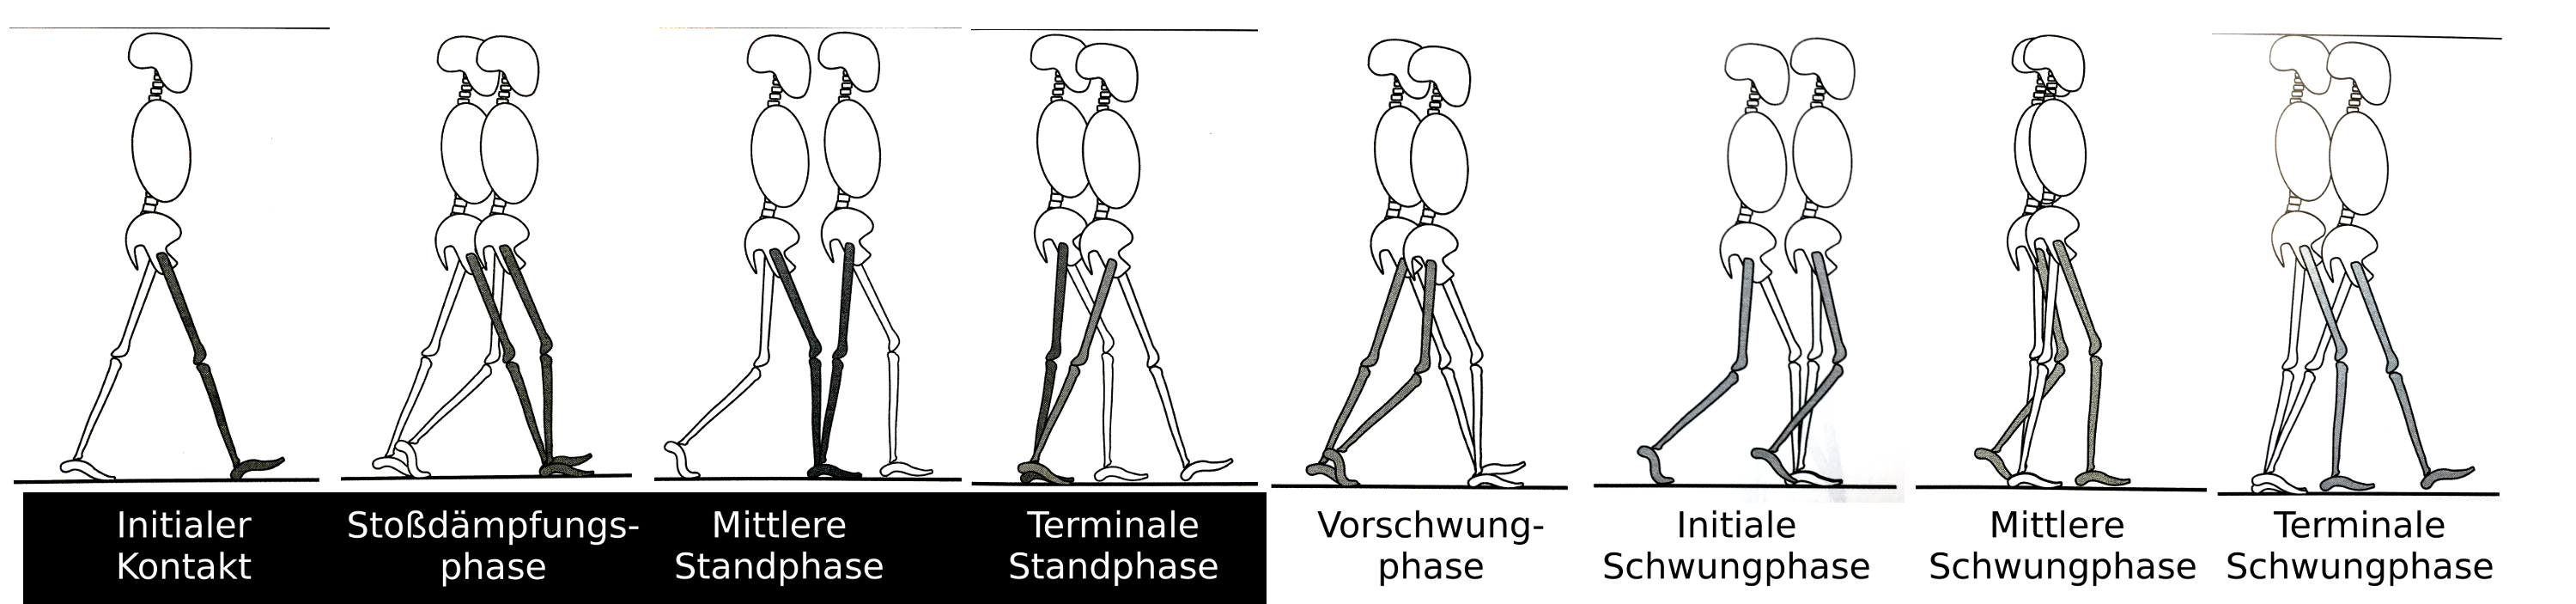
\includegraphics[width=\linewidth]{bilder/Einleitung/Skizze_Gangphasen_small}
	\caption[Gangphasen]{blabla blabla}
	\label{fig:Skizze_Phasen}
\end{figure}

\begin{figure}
	\centering
	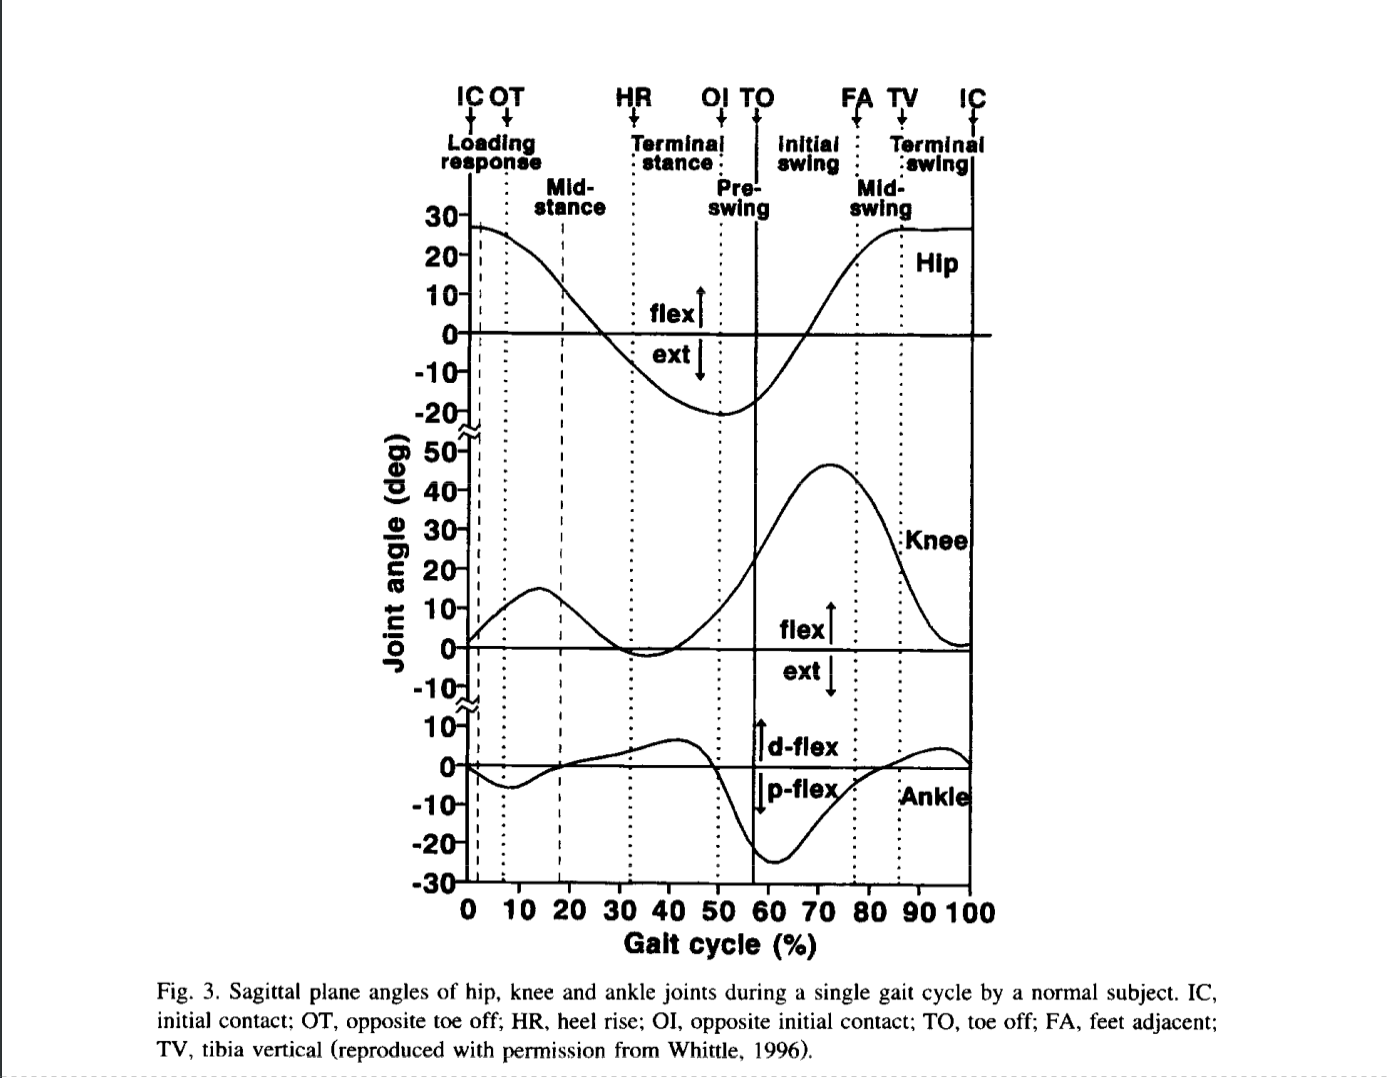
\includegraphics[width=0.7\linewidth]{bilder/Einleitung/gangphasen}
	\caption[Gangphasen]{blabla blabla}
	\label{fig:gangphasen}
\end{figure}


 Durch kinematische und kinetische Beobachtungen lassen sich diese 